\section{Advanced Tsay-Lee Framework}
\label{sec:advanced_tsay_lee_framework}

The work of Tsay and Lee \cite{TsayLee} was developed to ensure that even complex data structures like binary search trees could support lock-free properties while remaining linearizable. Simpler structures, such as linked lists, do not require such development; for instance, Heller et al. \cite{LockFreeList} achieved this by utilizing logical deletion. Non-blocking goal is to guarantee that at least one thread will infinitely often complete its data structure method execution. At the same time, we require these methods to be representable as atomic operations, preserving all partial execution orders. To achieve this, a frame-based approach was proposed. In this context, a frame is defined as a subtree section that originates at a specific node and is bounded below by a set of terminal nodes. The frame size corresponds to the number of elements it contains, encompassing all edges connecting the constituent nodes of the original tree. A frame is selected such that its complete atomic replacement preserves the internal invariants of the underlying data structure.

\usetikzlibrary{fit,positioning, backgrounds}

\begin{adjustbox}{max width=\linewidth, max height=\textheight, keepaspectratio}
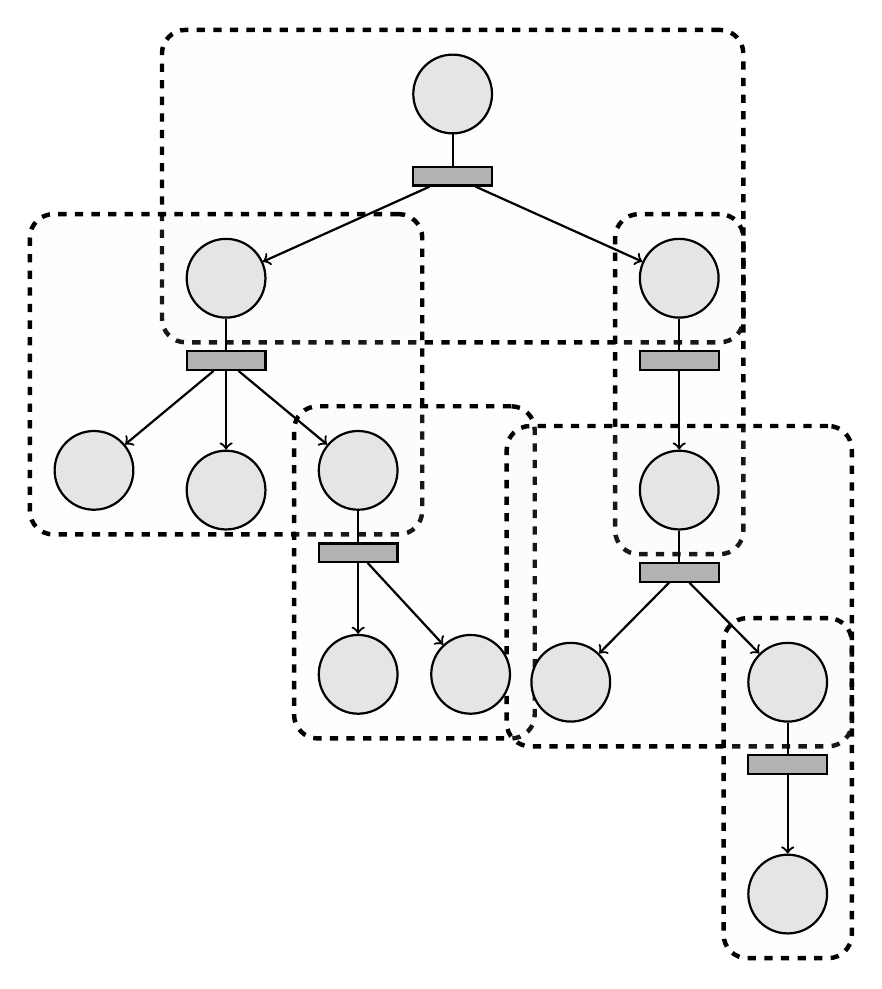
\begin{tikzpicture}[
    cNode/.style={circle, draw, minimum size=10mm, fill=black!10, thick, font=\small},
    sNode/.style={rectangle, draw, minimum width=10mm, minimum height=2mm, fill=black!30, thick},
    edge/.style={draw, thick},
    fStyle/.style={draw=black, ultra thick, dashed, fill=blue!5, fill opacity=0.1, rounded corners=3mm, inner sep=3mm}
]
    \node[cNode] (R) {};
    \node[sNode, below=0.4cm of R] (S) {};
    \path[edge] (R) -- (S);
    \node[cNode, below left=0.8cm and 2.0cm of S] (C1) {};
    \node[cNode, below right=0.8cm and 2.0cm of S] (C2) {};
    \path[edge] (S) edge[->] (C1) edge[->] (C2);
    \node[sNode, below=0.4cm of C1] (S1) {};
    \node[cNode, below left=0.9cm and 0.8cm of S1] (G1) {};
    \node[cNode, below=1.0cm of S1] (G2) {};
    \node[cNode, below right=0.9cm and 0.8cm of S1] (G3) {};
    \path[edge] (C1) -- (S1) (S1) edge[->] (G1) edge[->] (G2) edge[->] (G3);
    \node[sNode, below=0.4cm of G3] (S3) {};
    \node[cNode, below=0.9cm of S3] (GG1) {};
    \node[cNode, right=0.4cm of GG1] (GG2) {};
    \path[edge] (G3) -- (S3) (S3) edge[->] (GG1) edge[->] (GG2);
    \node[sNode, below=0.4cm of C2] (S2) {};
    \node[cNode, below=1.0cm of S2] (G4) {};
    \path[edge] (C2) -- (S2) (S2) edge[->] (G4);
    \node[sNode, below=0.4cm of G4] (S4) {};
    \node[cNode, below left=0.9cm and 0.5cm of S4] (GG3) {};
    \node[cNode, below right=0.9cm and 0.5cm of S4] (GG4) {};
    \path[edge] (G4) -- (S4) (S4) edge[->] (GG3) edge[->] (GG4);
    \node[sNode, below=0.4cm of GG4] (S5) {};
    \node[cNode, below=1.0cm of S5] (GGG1) {};
    \path[edge] (GG4) -- (S5) (S5) edge[->] (GGG1);

    \begin{scope}[on background layer]
    \node[fStyle, fit=(R) (S) (C1) (C2)] (F0) {};
    \node[fStyle, fit=(C1) (S1) (G1) (G3)] (F1) {};
    \node[fStyle, fit=(C2) (S2) (G4)] (F2) {};
    \node[fStyle, fit=(G3) (S3) (GG1) (GG2)] (F3) {};
    \node[fStyle, fit=(G4) (S4) (GG3) (GG4)] (F4) {};
    \node[fStyle, fit=(GG4) (S5) (GGG1)] (F5) {};
    \end{scope}
\end{tikzpicture}
\end{adjustbox}


The framework partitions the nodes accessed by each data structure operation into such frames. For example, to insert a node into the tree, the algorithm clones a frame that originates at the local root node. This frame encompasses several additional nodes required to guide the insertion operation as it traverses down the data structure. Thereafter, the target operation is either performed on these nodes or they remain unchanged; the frame is then atomically replaced, provided that no other concurrent thread has modified this specific set of nodes and edges. If a concurrent modification is detected, the transformation process is retried from scratch. Otherwise, as the operation traverses deeper, a new frame is allocated. This new frame is guaranteed to overlap with the previous one, ensuring that when it is replaced by its local copy, the nodes maintain their connectivity to the root and remain continuously accessible.

This implementation was designed for the DEC Alpha architecture \cite{SitesDECAlpha}, which allowed verification of whether another thread had modified a memory element. This capability is equivalent to executing multiple atomic load-linked/store-conditional (LL/SC) instructions. Modern computer architectures, however, lack such primitives; instead, the compare-and-swap (CAS) atomic operation is predominantly used. CAS accepts three arguments: the memory location to be updated, the expected value, and the desired new value. It possesses an infinite consensus number \cite{WaitFreeSync}, enabling non-blocking synchronization for an infinite number of threads. If a thread fails to update the value due to a mismatch with the expected value, CAS returns false and no replacement occurs; otherwise, the function returns true.

Based on these operations, Natarajan et al. \cite{WaitFreeBST} proposed decomposing vertices and their subtrees into distinct, interconnected nodes. Under this approach, to atomically replace a frame with its local copy, a CAS operation needs to be executed only on the single vertex from which all other vertices in that subtree section are reachable. This unique vertex serves as the root of the frame. If the CAS on the root fails, it implies that another concurrent thread has modified it first, requiring the current thread to either retry the execution or raise an error.

However, a critical issues arises if a concurrent thread executes a CAS on an internal node rather than the frame root, compromising consistency. This internal update cannot detect the root-level CAS that replaces the entire frame. Consequently, the concurrent thread becomes disconnected from the active topology, as its target nodes are permanently bypassed by the new local frame copy. To prevent this isolation, method descriptors were introduced.

To execute an operation, a thread creates a descriptor encapsulating its current data structure operation. Afterwards, a reference to this descriptor is attached to all nodes involved in the operation. If another thread attempts to access a marked node, it must first inspect the descriptor and help the original thread complete its execution. This helping mechanism must be applied recursively if executing the helping operation requires assisting a third operation, and so on. This helping mechanism, akin to the multi-word CAS approach by Ellen et al. \cite{NonBlockBST}, ensures both system-wide progress and strict linearizability \cite{Linearizability} during concurrent modifications.

We formalize this frame-based update in TLA+ to ensure its correctness. The \texttt{TreeCAS} module is modeled around a minimal tree consisting of a root and its child leaf. This structure is sufficient to verify the framework's correctness, as the critical race condition to evaluate involves a larger frame overlapping a smaller one. Furthermore, scaling the state space to include more nodes does not break the framework, as confirmed by our larger-scale model checking runs. The only part of the spec needs to replace is \texttt{InitialTree} internal variable in \texttt{Init} statement (Except for \texttt{Nodes} in config file).

The model state is mainly defined by variables: \texttt{nodeStruct} and \texttt{structLinks} map nodes to their internal structures and target child nodes; \texttt{nodeDesc} tracks descriptor references (or \texttt{NULL}) within cells; \texttt{descState} manages the descriptor lifecycle (\texttt{IDLE}, \texttt{ACTIVE}, \texttt{COMMITTING}, \texttt{SUCCESS}, \texttt{ABORTED}); and \texttt{descPending} along with \texttt{descFrame} track unacquired nodes and assigned frame boundaries for each descriptor.

To model the allocation of new nodes, we utilize an infinite memory pool constrained by a state-space filter limiting the maximum number of active allocated cells to 6. The overall algorithm comprises 5 distinct phases, with the 3rd phase implementing the recursive helping mechanism. This phase is structured as follows:

\begin{tla}
(* Cooperatively advance for descriptor if it blocks our path *)
Help(d, n) == LET otherD == nodeDesc[n] IN
  /\ descState[d] = "ACTIVE" (* We can only offer help if *)
  /\ n \in descPending[d]    (* we are actively trying to acquire nodes *)
  /\ nodeDesc[n] /= NULL (* The target node must be currently *)
  /\ nodeDesc[n] /= d    (* locked by a different descriptor otherD *)
  /\ IF descState[otherD] \in {"ACTIVE", "COMMITTING"}
     THEN (* If the competitor is in progress *)
        CommitStep(otherD)
     ELSE IF descState[otherD] \in {"SUCCESS", "ABORTED"}
     THEN (* Help it unlock nodes and free memory *)
        ReleaseDescriptor(otherD)
     ELSE (* If otherD is IDLE, do nothing *)
        UNCHANGED vars
\end{tla}
\begin{tlatex}
\@x{}%
\@y{%
  Cooperatively advance for descriptor if it blocks our path 
}%
\@xx{}%
 \@x{ Help ( d ,\, n ) \.{\defeq} \.{\LET} otherD \.{\defeq} nodeDesc [ n ]
 \.{\IN}}%
\@x{\@s{8.2} \.{\land} descState [ d ] \.{=}\@w{ACTIVE}}%
\@y{%
  We can only offer help if 
}%
\@xx{}%
\@x{\@s{8.2} \.{\land} n \.{\in} descPending [ d ]}%
\@y{%
  we are actively trying to acquire nodes 
}%
\@xx{}%
\@x{\@s{8.2} \.{\land} nodeDesc [ n ] \.{\neq} NULL}%
\@y{%
  The target node must be currently 
}%
\@xx{}%
\@x{\@s{8.2} \.{\land} nodeDesc [ n ] \.{\neq} d}%
\@y{%
  locked by a different descriptor otherD 
}%
\@xx{}%
 \@x{\@s{8.2} \.{\land} {\IF} descState [ otherD ] \.{\in} \{\@w{ACTIVE}
 ,\,\@w{COMMITTING} \}}%
\@x{\@s{8.2} \.{\THEN}}%
\@y{%
  If the competitor is in progress 
}%
\@xx{}%
\@x{\@s{20.5} CommitStep ( otherD )}%
 \@x{\@s{8.2} \.{\ELSE} {\IF} descState [ otherD ] \.{\in} \{\@w{SUCCESS}
 ,\,\@w{ABORTED} \}}%
\@x{\@s{8.2} \.{\THEN}}%
\@y{%
  Help it unlock nodes and free memory 
}%
\@xx{}%
\@x{\@s{20.5} ReleaseDescriptor ( otherD )}%
\@x{\@s{8.2} \.{\ELSE}}%
\@y{%
  If otherD is IDLE, do nothing 
}%
\@xx{}%
\@x{\@s{20.5} {\UNCHANGED} vars}%
\end{tlatex}

As demonstrated here, we do not distinguish between the concept of an execution thread and the descriptor of the operation it performs. This abstraction can be interpreted as the use of coroutines within the physical production code, a pattern that is prevalent in practice. An interesting aspect of constructing formal specifications for non-blocking algorithms is that the \texttt{Help(d, n)} routine is only strictly necessary in the actual implementation. While omitting it compromises the global progress property, it is not mathematically required to maintain safety invariants.

\begin{tla}
GlobalProgress ==
  \E d \in Descs : descState[d] = "ACTIVE" ~>
    \E u \in Descs : descState[u] = "SUCCESS"
      \/ ~FreeStructConstraint
\end{tla}
\begin{tlatex}
\@x{ GlobalProgress \.{\defeq}}%
 \@x{\@s{8.2} \E\, d \.{\in} Descs \.{:} descState [ d ] \.{=}\@w{ACTIVE}
 \.{\leadsto}}%
\@x{\@s{16.4} \E\, u \.{\in} Descs \.{:} descState [ u ] \.{=}\@w{SUCCESS}}%
\@x{\@s{24.59} \.{\lor} {\lnot} FreeStructConstraint}%
\end{tlatex}

To verify linearizability, we enforced the preservation of the tree topology invariant, ensuring that every node remains continuously reachable from the root and is never erroneously obscured by a concurrent transaction.

Another aspect of the specification is the CAS acquisition phase. If the linked structure of a target node has been modified, our transaction must be aborted. The core block for this mechanism is presented below.

\begin{tla}
/\ IF nodeStruct[n] /= descExpectedStruct[d][n]
  THEN (* The underlying node structure has changed since *)
       (* the descriptor creation. Abort the transaction. *)
    /\ descState' = [descState EXCEPT ![d] = "ABORTED"]
    /\ UNCHANGED vars \ {...}
  ELSE IF nodeDesc[n] = NULL
  THEN (* CAS SUCCESS: Lock the node *)
    ExecuteAcquire(d, n)
  ELSE (* CAS FAIL: Node is occupied *)
    UNCHANGED vars
\end{tla}
\begin{tlatex}
 \@x{ \.{\land} {\IF} nodeStruct [ n ] \.{\neq} descExpectedStruct [ d ] [ n
 ]}%
\@x{\@s{8.2} \.{\THEN}\@s{8.2}}%
\@y{%
  The underlying node structure has changed since 
}%
\@xx{}%
\@x{\@s{16.4}}%
\@y{%
  the descriptor creation. Abort the transaction. 
}%
\@xx{}%
 \@x{\@s{16.4} \.{\land} descState \.{'} \.{=} [ descState {\EXCEPT} {\bang} [
 d ] \.{=}\@w{ABORTED} ]}%
\@x{\@s{16.4} \.{\land} {\UNCHANGED} vars \.{\,\backslash\,} \{ \.{\dots} \}}%
\@x{\@s{8.2} \.{\ELSE} {\IF} nodeDesc [ n ] \.{=} NULL}%
\@x{\@s{8.2} \.{\THEN}}%
\@y{%
  CAS SUCCESS: Lock the node 
}%
\@xx{}%
\@x{\@s{16.4} ExecuteAcquire ( d ,\, n )}%
\@x{\@s{8.2} \.{\ELSE}}%
\@y{%
  CAS FAIL: Node is occupied 
}%
\@xx{}%
\@x{\@s{16.4} {\UNCHANGED} vars}%
\end{tlatex}
